\documentclass[12pt,a4paper]{article}

\usepackage[left=2cm,text={17cm,24cm},top=3cm]{geometry}
\usepackage[english]{babel}
\usepackage[utf8]{inputenc}
\usepackage[T1]{fontenc}

\usepackage{url}
\usepackage{float}
\usepackage{amsthm}
\usepackage{comment}
\usepackage{csquotes}
\usepackage{etoolbox}
\usepackage{graphicx}
\usepackage{hyperref}
\usepackage{tocloft}

\def\UrlBreaks{\do\/\do-\do\&\do=\do\_\do?} % URL breaking characters

\newcommand{\red}[1]{\textcolor{red}{#1}} % \red{text in red}
\newcommand{\blue}[1]{\textcolor{blue}{#1}} % \blue{text in blue}
\newcommand{\TODO}{\textbf{\textcolor{red}{TODO}}} % red bold TODO
\newcommand{\tilda}{\raisebox{0.5ex}{\texttildelow}} % command \tilda for '~' character
\newcommand{\uv}[1]{``#1''}

\renewcommand{\cftdot}{} % remove dots ([sub]secion ......... number) from table of contents
\renewcommand{\baselinestretch}{1.1}

\theoremstyle{definition}
\newtheorem{definition}{Definition}[section]
\graphicspath{{img/}} % path to images
\patchcmd{\thebibliography}{\section*{\refname}}{}{}{} % do not create section for bibliography
\hypersetup{
    linktoc    = all,
    colorlinks = true,
    citecolor  = green,
    linkcolor  = red,
    urlcolor   = blue,
}

\begin{document}

\begin{titlepage}

    \begin{center}
        % FIX: lines must end with '%', if not then it will result in an incorrect centering
        \vfill {%
            \Huge{%
                \textsc{%
                    Faculty of Informatics\\[3mm]%
                    Masaryk University%
                }%
            }%
        }%

        \hfill\\[15mm]

        \begin{figure}[!h]
            \centering
            
\includegraphics[scale=3]{img/muni-fi-logo.pdf}
        \end{figure}

        \hfill\\[10mm]

        \Huge{
            \textbf{
                IV064
            }
        }

        \hfill\\[-10mm]

        \huge{
            \textbf{
                Information Society
            }
        }

        \hfill\\[10mm]

        \LARGE{
            \textbf{
                Modern Agile Software Engineering
            }
        }
        \vfill

    \end{center}

        \Large{
            \noindent Adrián Tóth (491322)\hfill \today
        }

\end{titlepage}

\setlength{\parskip}{0pt}
    {
        \hypersetup{
            hidelinks=true
        }
        \tableofcontents
    }
\setlength{\parskip}{0pt}

\newpage

\section{Software Engineering}

    From time to time, software engineering become the most important part of software development. There are many different definitions of software engineering which are sometimes misleading and incorrect. The \textit{IEEE}\footnote{Institute of Electrical and Electronics Engineers} defines the software engineering, which clarifies its true meaning in the software development.

    \begin{definition}
        Software engineering\\[-5mm]
        \begin{center}
            \begin{minipage}{0.9\textwidth}
                The application of a systematic, disciplined, quantifiable approach to the development, operation, and maintenance of software; that is, the application of engineering to software~\cite{182763}.\\[-2.5mm]
            \end{minipage}
        \end{center}
    \end{definition}

    Up to the present time, software engineering has evolved and adapted by the time, introducing new methodologies for software development, which lead to an increase in the number of successful projects. Software development methodologies provide a framework for planning, executing, and managing the process of developing software systems~\cite{7006383}. The importance of software engineering has resulted in a research of software engineering itself in a form of empirical, contemplative, case and other studies, which delivered new approaches, attitudes and practices. The speed of information technology development is massively progressive and incredibly fast and it is also part of our daily life.

    \begin{definition}
        Delivery\\[-5mm]
        \begin{center}
            \begin{minipage}{0.9\textwidth}
                Release of a system or component to its customer or intended user~\cite{182763}.\\[-2.5mm]
            \end{minipage}
        \end{center}
    \end{definition}

    Nowadays requirements for the software are unbearably high. Developing a software present days means, to deliver the product as soon as possible and simultaneously provide the best possible product quality, which is classified by product metrics. Quality plays a vital role for the software users~\cite{8748529}. This article deals with the software delivery time from the view of the modern software engineering.\\

    Developing a quality software product is an essential need for the software industry~\cite{8748529}. To deliver a quality product under short time, it requires development agility, cross-functional teams and collaborative effort of self-organization. To deliver a quality product as fast as possible, it is needed to meet the above mentioned requirements and use a proper framework and methodology. The most common development methodologies is agile as well as predictive methodology. In addition to agile development methodology, we will discuss and compare the newly integrated methodologies and practices.

    \subsection{Time to Market}

        Time to the market is the key to success in the field of information technology. Businesses must be prepared and shaped to adapt and evolve the modern breakthrough technologies. It is not so easy to be up to date, especially not in the information technology business. From time to time, as every manual tasks were transformed into a fully automated hands--off processes, the software engineered was also influenced by this automation impact. Automation is limitless because of the fact that there can be any task transfered from manual to automated. If the automated process is configured properly, it may save a huge amount of time.\\

        The software development must be also faster, the automation of the software delivery pipeline is not the only one required for a quick software delivery. Time needed for software product creation is the most influencing part of the delivery time. Based on the development progress the time may be also prolonged or shortened.

\section{Agile Development}

    Delivering a product in the shortest possible time requires good software development methodology, which is possible with agile development methodology. Agile methodology provides all the necessary approaches, practices and disciplines to the software development, which allow fast product delivery and high quality of the product. The main and principal approaches to software development are: flexible and adaptable, focus on people (customers, users, developers), regularly updated requirements. In a comparison to predictive methodology, agile provides less (minimal) effort to upfront planning and the product is delivered after small iterations in a form of product increments (releases). Agile methods are based on small development cycles, continuous integration of software versions, adaptive planning, team collaboration, customer involvement, and feedback~\cite{YOUNAS2018142}.

    \begin{definition}
        Scrum\\[-5mm]
        \begin{center}
            \begin{minipage}{0.9\textwidth}
                A framework within which people can address complex adaptive problems, while productively and creatively delivering products of the highest possible value~\cite{ScrumOrgGuide}.\\[-2.5mm]
            \end{minipage}
        \end{center}
    \end{definition}

    SCRUM is the most well known and common agile software development framework. It is simple to understand but difficult to master. The framework describes and defines the whole development structure -- events, roles and artifacts. The scrum framework poster in Figure~\ref{fig:ScrumOrgPoster} provides a graphical view of how scrum is implemented at a team level within an organization~\cite{ScrumOrgPoster}.\\

    It is difficult to state precisely the advantages and disadvantages against agile alternatives. Both agile and predictive have pros and cons which can differ by the project requirements. Predictive approach is greatly used for a project where we exactly know the product requirements and specifications. Agile approach is useful while it is needed to deliver the product (or maybe its prototype) in the quickest time while it might be later enhanced by additional patches via updates. The manner of time and product specifications (requirements definition) are crucial to state the shortcomings of each methodologies.

    \subsection{DevOps}

    A new development methodology has been created to reduce the time costs for software product delivery. You likely have heard of the word DevOps, so let us clarify its true meaning. The modern software development involves an immense effort to the product deployment because of integration and connection conflicts between each product parts. DevOps efficiently integrates development, delivery, and operations, thus facilitating a lean, fluid connection of these traditionally separated silos~\cite{7458761}. It came to address this conflict and bridge the gap between developers and operations staff~\cite{7339039}.

    \begin{definition}
        DevOps\\[-5mm]
        \begin{center}
            \begin{minipage}{0.9\textwidth}
                DevOps is an organizational approach that stresses empathy and cross-functional collaboration within and between teams~--~especially development and IT operations~--~in software development organizations, in order to operate resilient systems and accelerate delivery of changes.~\cite{7169442}.\\[-2.5mm]
            \end{minipage}
        \end{center}
    \end{definition}

    The acronym consists from two parts Dev and Ops. DevOps is an abbreviation of development and IT operations, it is not limited to those two teams; thus, there is no need for "extending" acronyms like DevSecOps or DevNetOps~\cite{7169442}.

    \begin{figure}[H]
        \centering
        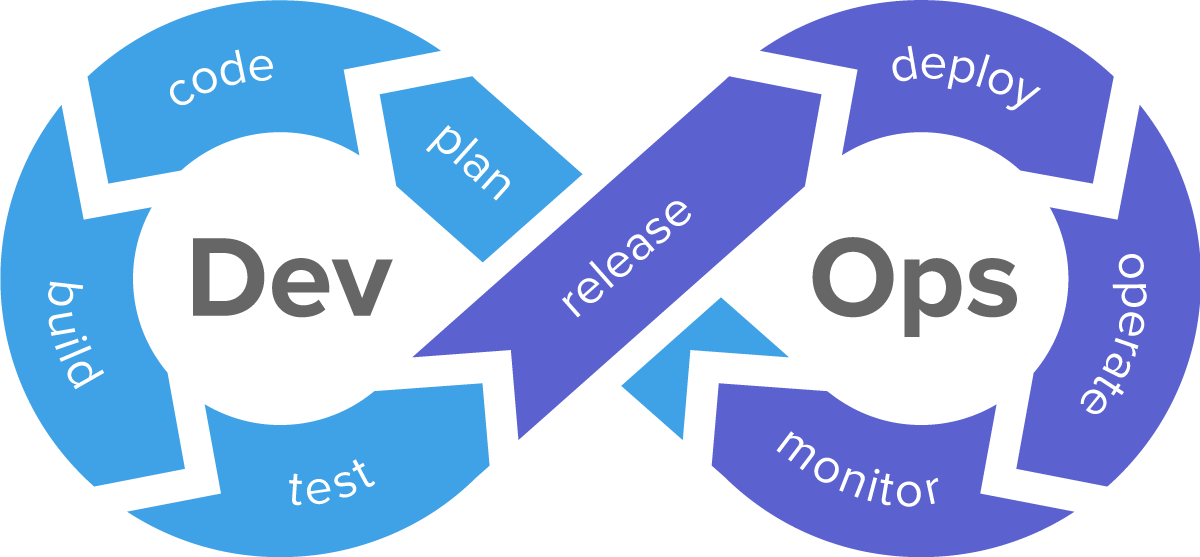
\includegraphics[scale=0.25]{img/devops.png}
        \caption{DevOps environment~\cite{devops1}.}
        \label{fig:devops}
    \end{figure}

    For the purpose of development acceleration, the DevOps is fundamental to agile development. The above stated facts point to that it provides an automated way how to deliver product as fast as possible, which may be also included in other types of developments. Under those circumstances, as the actions are done in a non manual way after each other, we denote this process as continuous. DevOps uses many continuous approaches, the most important one from the all of them is continuous delivery which will be described later in the following Section~\ref{sec:CD}.\\

    All things considered, DevOps has a very beneficial influence for the development itself. It results in time costs reduction for the product delivery -- from source code change to a deployable usable release. Obviously, DevOps must be performed by somebody so as a disadvantage, we may consider that the development requires a special team for this purpose.

\section{Continuous Delivery}\label{sec:CD}

    Continuous delivery advocates claim that it lets organizations rapidly, efficiently, and reliably bring service improvements to market and eventually stay a step ahead of the competition~\cite{cd-book}.

    \begin{definition}
        Continuous Delivery\\[-5mm]
        \begin{center}
            \begin{minipage}{0.9\textwidth}
                Continuous Delivery (CD) is a software engineering approach in which teams keep producing valuable software in short cycles and ensure that the software can be reliably released at any time~\cite{8452107}.\\[-2.5mm]
            \end{minipage}
        \end{center}
    \end{definition}

    Continuous delivery is related to the DevOps automation. Using a continuous delivery approach is very powerful and useful to the development. Implementing a continuous delivery into the development process requires a continuous delivery pipeline configuration and setup. The pipeline must implement altogether the development actions such as build, test, release, deploy in an automated process. Figure~\ref{fig:cd} as an illustrating image visualize the order of main actions from high perspective required for the implementation.

    \begin{figure}[H]
        \centering
        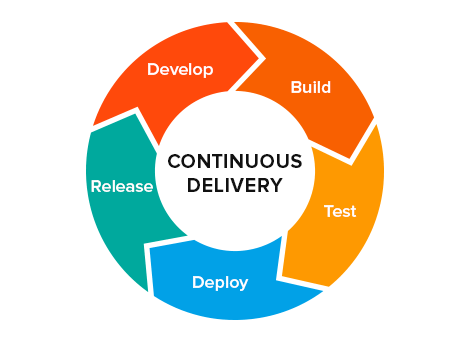
\includegraphics[scale=0.5]{img/cd.png}
        \caption{Continuous delivery workflow~\cite{cd1}.}
        \label{fig:cd}
    \end{figure}

    In conclusion, continuous delivery is a software development discipline where you build software in such a way that the software can be released to production at any time~\cite{cd2}. Continuous delivery can bring huge benefits, but implementing continuous delivery is challenging~\cite{8452107}. Development needs extra time for the continuous delivery pipeline implementation and later, maintenance and further support for additional changes necessary to adapt to the pipeline. Excluding the implementation and maintenance, the result of using a continuous delivery is very beneficial and advantageous. The main advantage of that it is an instant problem detection for such problems as dependency errors between each part of product, which result in a broken pipeline where the developers can respond quickly to that problems.\\

    Continuous delivery involves continuous integration, continuous testing, continuous deployment, continuous monitoring and continuous pipeline. There are the key parts of continuous delivery which need special attention to. We are going to discuss the basic principles and fundamentals as well as pros and cons in the following sections below about the most important parts -- continuous integration and the pipeline itself.

    \subsection{Continuous Integration}

        As part of agile transformation in past few years we have seen IT organizations adopting continuous integration principles in their software delivery lifecycle, which has improved the efficiency of development teams~\cite{7173368}. The modern software development is using enterprise architectural design patterns which divides the system to subsystem based on its functional purpose and operation. Subsystem set (each function independent parts) of the whole system must be integrated into one system unit which is not as easy as it looks. To describe what continuous integration is, we must declare some terms for better understanding.

        \begin{definition}
            Build\\[-5mm]
            \begin{center}
                \begin{minipage}{0.9\textwidth}
                    A Build may refer to a set of activities performed to generate, test, inspect, and deploy software~\cite{ci1}.\\[-2.5mm]
                \end{minipage}
            \end{center}
        \end{definition}

        \begin{definition}
            Integration Build\\[-5mm]
            \begin{center}
                \begin{minipage}{0.9\textwidth}
                    An Integration Build is the act of combining software components (programs and files) into a software system~\cite{ci1}.\\[-2.5mm]
                \end{minipage}
            \end{center}
        \end{definition}

        In brief, the integration build is a transformation process that integrate these software components together into a one unified entity. It does depend where it is done. If a developer wants to run the software on his local machine, he will probably perform a private integration build. In contrast, the pure integration build is mostly performed on some remote system after which, the system entity may pass to the following stages -- system testing, deployment or release.

        \begin{definition}
            Continuous Integration\\[-5mm]
            \begin{center}
                \begin{minipage}{0.9\textwidth}
                    Continuous Integration (CI) is a development practice that requires developers to integrate code into a shared repository several times a day~\cite{thoughtworks}.\\[-2.5mm]
                \end{minipage}
            \end{center}
        \end{definition}

        Martin Fowler pointed out the problem of subsystem integration in his article: \uv{I was told that this project had been in development for a couple of years and was currently integrating, and had been integrating for several months.}~\cite{ci2}. Some research articles distinguish integrations types into two groups~--~big bang integration and daily integration. The most common one is the daily integration because its alternative -- big bang integration, does not reduce the risks introduced during the system unification. The daily integration, as it is stated in the name, provides periodical integrations, which lead to less conflicts and risks reduction between system parts.

        \begin{figure}[H]
            \centering
            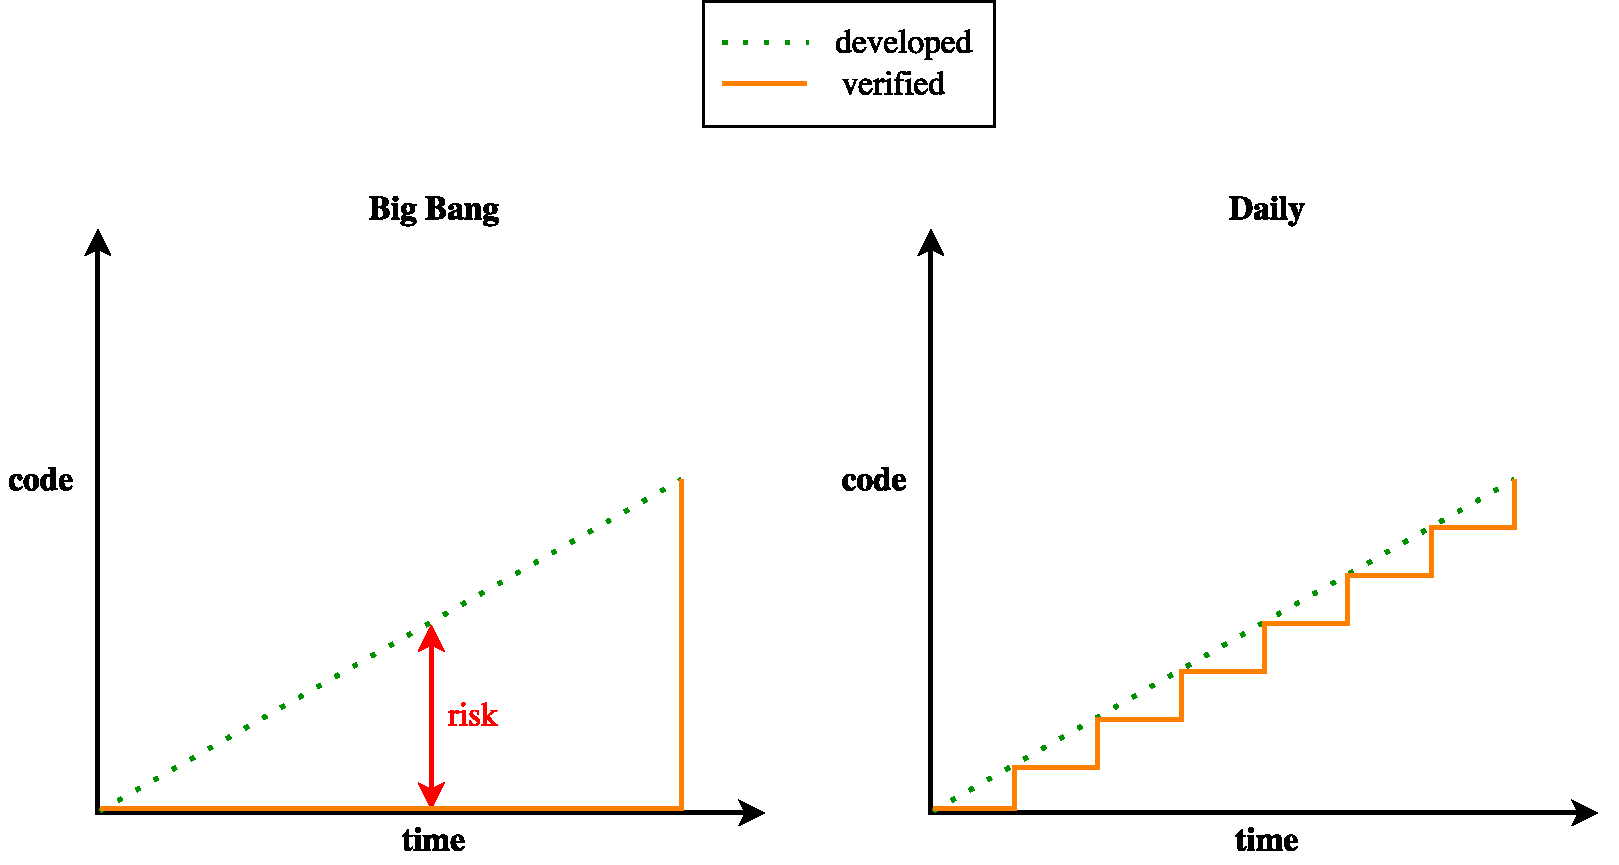
\includegraphics[scale=0.5]{img/big_bang_vs_daily_build.pdf}
            \caption{Comparison of integration builds~\cite{FITMT21007}.}
            \label{fig:cd}
        \end{figure}

        \begin{displayquote}
            \textit{\uv{Not integrating continuously is expensive. If you don’t follow a continuous approach, you’ll have longer periods between integrations. This makes it exponentially more difficult to find and fix problems. Such integration problems can easily knock a project off-schedule, or cause it to fail altogether.}}\\[-2em]
            \begin{flushright}
                -- ThoughtWorks$^{\tiny{\textregistered}}$~\cite{thoughtworks}
            \end{flushright}
        \end{displayquote}

        A continuous integration system is often considered one of the key elements involved in supporting an agile software development and testing environment~\cite{5261055}. There are few practices~\cite{ci2} that is good to follow while using continuous integration, which are listed below.\\[-4mm]

        \begin{itemize}
            \item Use and maintain a single source code repository.\\[-8mm]
            \item Automate the build.\\[-8mm]
            \item Make the build self-testing.\\[-8mm]
            \item Everyone commits to the mainline every day.\\[-8mm]
            \item Every commit should build the mainline on an integration machine.\\[-8mm]
            \item Fix broken builds immediately.\\[-8mm]
            \item Keep the build fast.\\[-8mm]
            \item Test in a clone of the production environment.\\[-8mm]
            \item Make it easy for anyone to get the latest executable.\\[-8mm]
            \item Everyone can see what's happening.\\[-8mm]
            \item Automate deployment.\\[-4mm]
        \end{itemize}

        The continuous integration pros and cons are most likely same as what was mentioned in paragraph 3 of Section~\ref{sec:CD}. The trouble with deferred integration is that it's very hard to predict how long it will take to do, and worse it's very hard to see how far you are through the process~\cite{ci2}. While using a continuous approach to the integrations we completely erase the problem of later integration what is considered as a main advantage for using continuous integration.

    \subsection{Deployment Pipeline}


\newpage

\section{References}
\bibliographystyle{englishiso}
\begin{flushleft}
    \bibliography{quotation}
\end{flushleft}

\newpage

\section{Appendix}

    \begin{figure}[H]
        \centering
        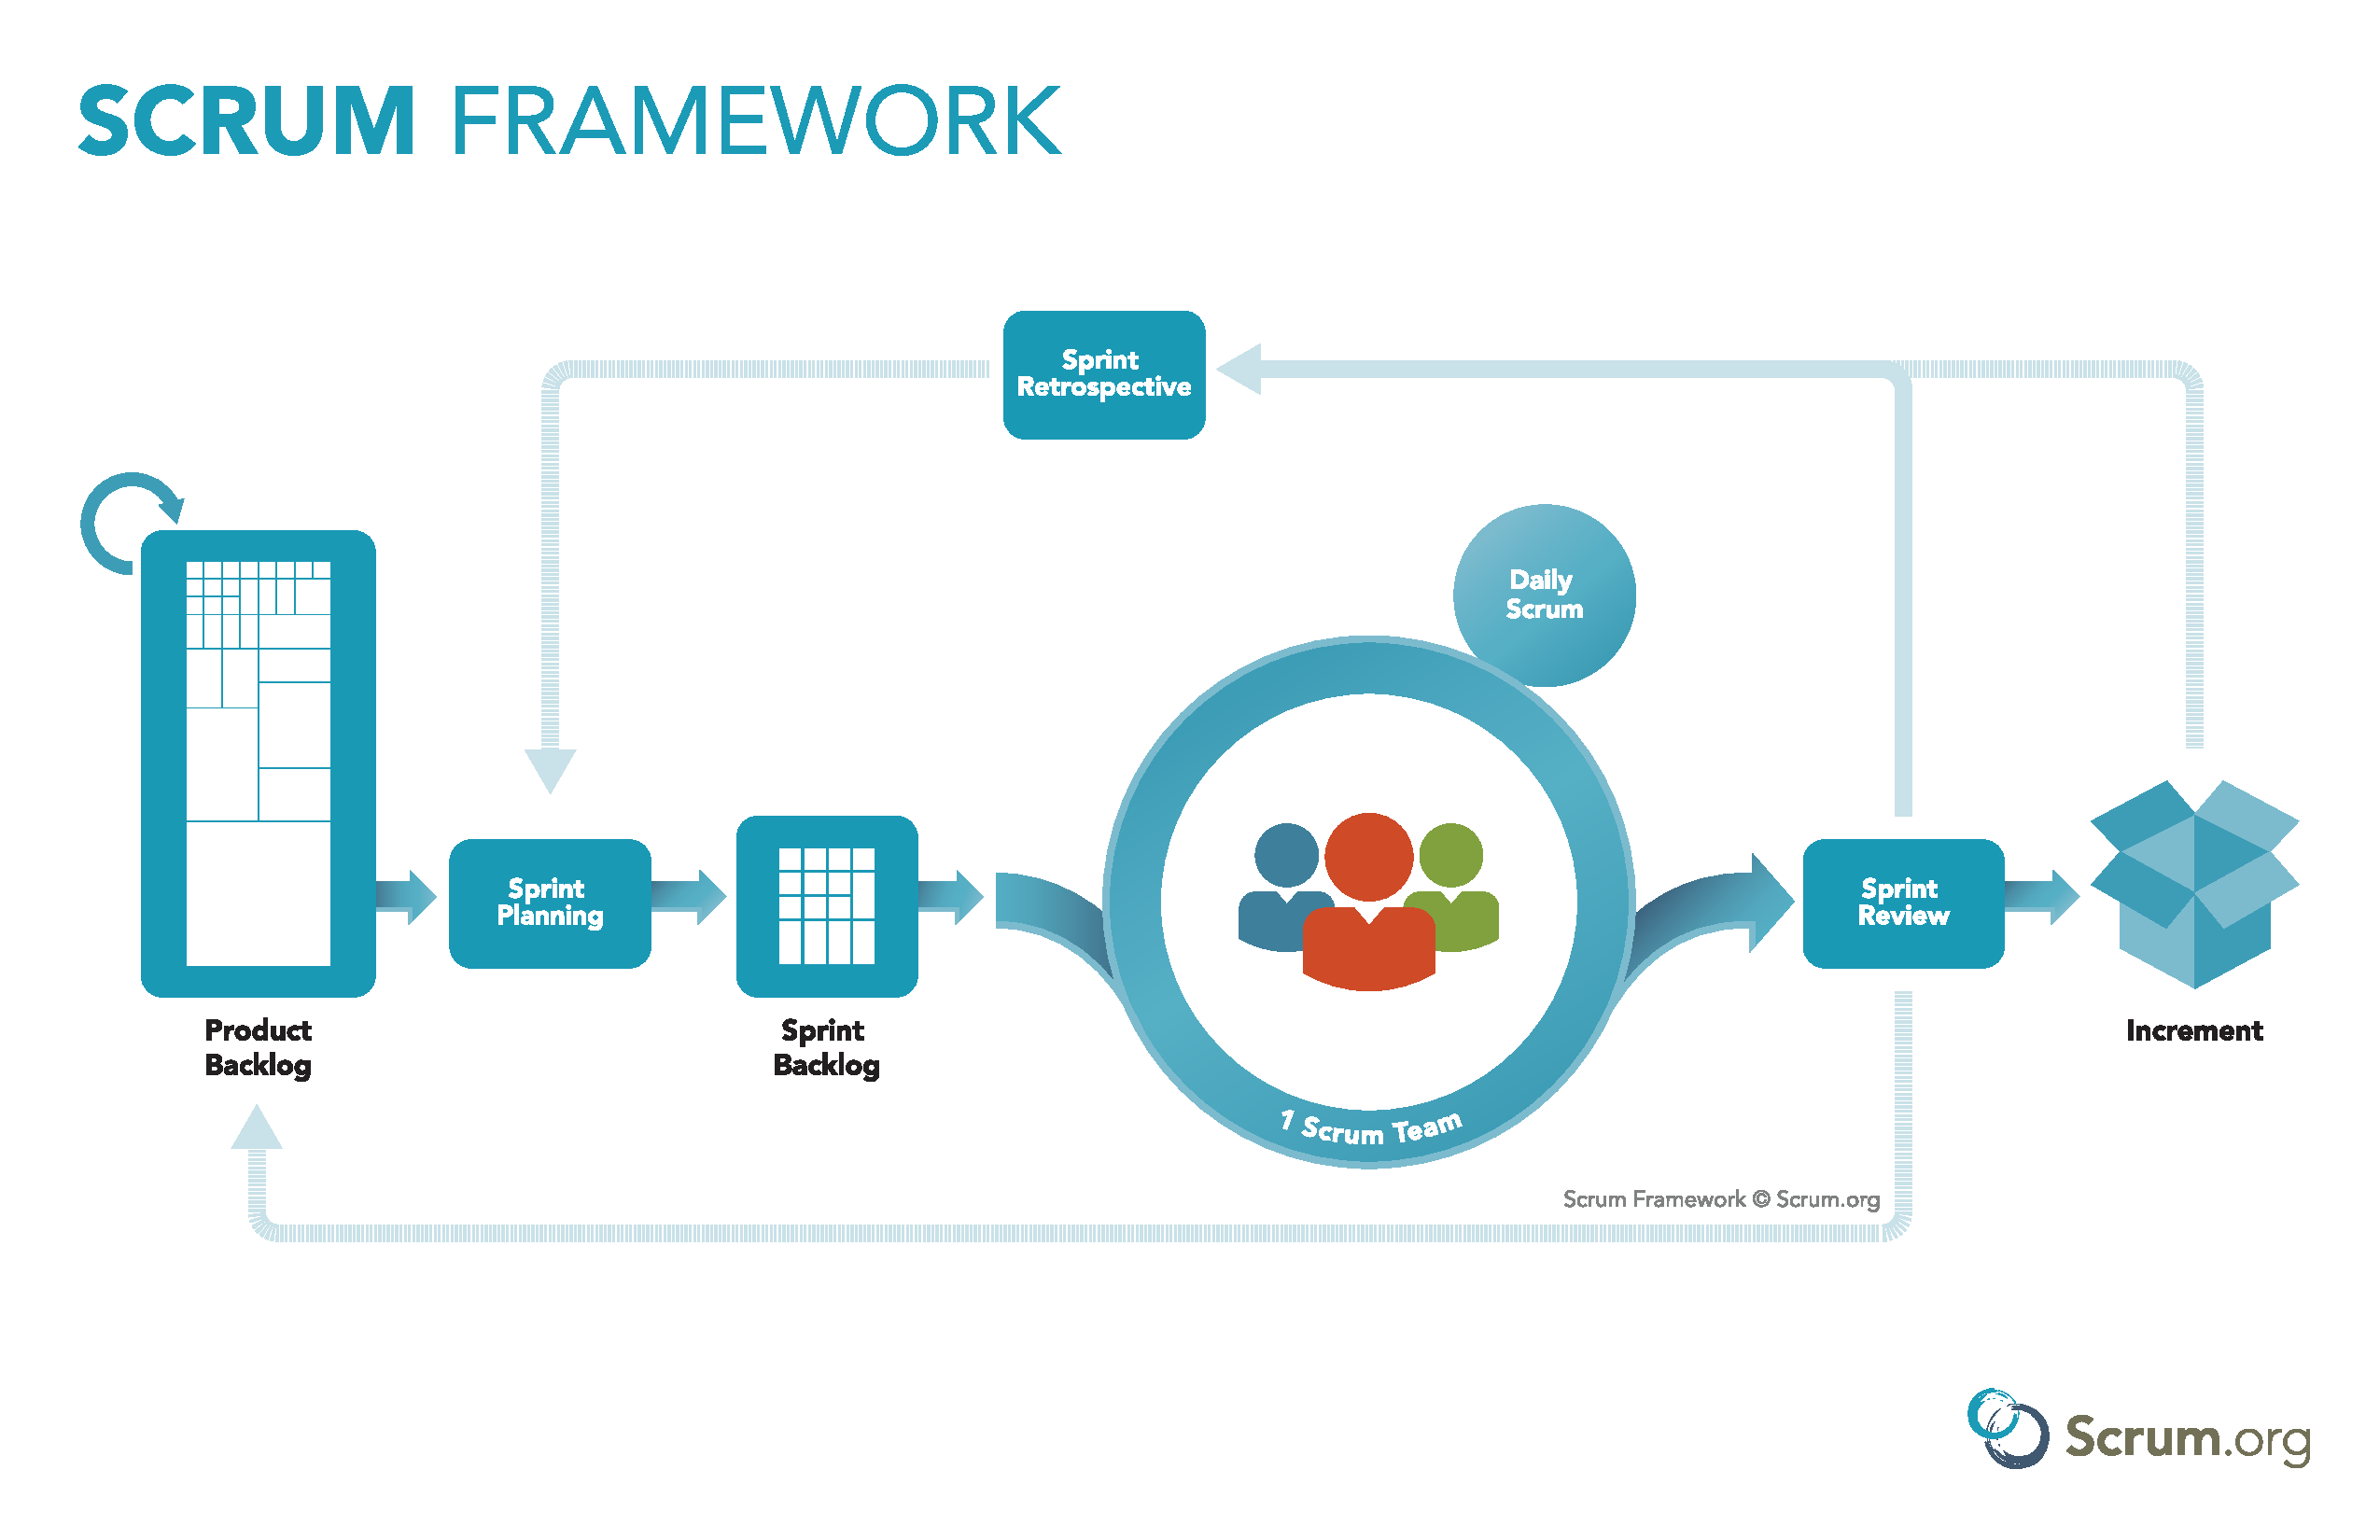
\includegraphics[scale=0.4]{img/ScrumFramework.pdf}
        \caption{The Scrum Framework Poster~\cite{ScrumOrgPoster}.}
        \label{fig:ScrumOrgPoster}
    \end{figure}

\end{document}
